\section{Evaluation}
\label{sec:eval}

We first introduce the datasets
and the experimental setup. 
We design two experiments, 
\textbf{general length control} and \textbf{zero-shot length control},
to compare our approach with baselines.~\footnote{Data and source code are 
available at: \url{https://github.com/YizhuLiu/lengthcontrol}.}
General length control experiment trains and tests the models on 
the entire original dataset.
Zero-shot length control experiment tests the model on 
a subset of the test set 
whose summary lengths fall within a certain range,
and trains the model on training data with summary lengths outside this range.
In each of the two experiments, we evaluate methods' ability to do
\textbf{length control} and 
\textbf{information selection}.

\subsection{Datasets}
We use two popular summarization datasets.
\textbf{CNN/Daily Mail}
(CNNDM)~\cite{HermannKGEKSB15}
consists of pairs of a single source document and a multi-sentence summary.
The dataset includes 286,817 training pairs,
13,368 validation pairs and 11,487 test pairs.
\textbf{XSUM}~\cite{XSUM} is composed of article and 
single-sentence summary pairs. 
The number of samples in training/validation/test sets 
are 204,045/11,332/11,334.

\subsection{Baselines}
The existing length-controllable models with good performance are 
listed in \tabref{tab:baselines}. 

\begin{table}[th]
	\scriptsize
	\centering
	\begin{tabular}{|m{1.0cm}<{\raggedleft}|p{5.6cm}|}
		\hline
		\textbf{Abbrev.} & \textbf{Description} \\ 
		\hline
		Exact & \tabincell{l}{Ignore $eos$ before generated summary within the desired \\ length and insert $eos$ at the desired length.} \\
		\hline 
		LenEmb & Input remaining length.~\cite{KikuchiNSTO16} \\
		\hline
		LC & Take desired length as input.~\cite{LiuLZ18}\\
		\hline
		GOLC & Apply length-aware loss.~\cite{GOLC19} \\
		\hline
		LenAtten &Add length attention unit.~\cite{lenatten21} \\
		\hline
		LPAS & Extract prototype summary.~\cite{Proto20}\\
		\hline
		BLPAS & Apply Prot on top of BART\\
		\hline
	\end{tabular}
	\caption{The abbreviation and description of methods.}
	\label{tab:baselines}
\end{table}

In the experiments, LAAM and PtLAAM
are implemented on top of BART\footnote{In rest of this paper, LAAM refers 
to BART using LAAM as cross-attention, for simplicity.},
because BART~\cite{BART19} is one of the SOTA models in summarization,
and it uses less memory and training time than its peers~\cite{analysis20}.  
Exact is not a summarization model but is used here to achieve hard
length control on any seq2seq models to produce summaries of exact lengths.  

\subsection{Experimental Setup}
\label{sec:expset}
We follow~\citet{LiuLZ18} and \citet{Proto20}
to segment datasets by different length ranges
and set the discrete bins $B$ of summary length ranges in \secref{sec:lbd}.
The $B$ of CNNDM is $B_{c}=\left\{(0,10],(10,30],...,(90,+\infty)\right\}$ and that of XSUM is $B_{x}=\left\{(0,10],(10,30],(30,+\infty)\right\}$.
\footnote{
Because historically, to test length control abilities,
the test sets of the datasets are split into some predefined ranges,
in this work, we adopt the same ranges in creating the bins.} 
$B_x$ has only 3 ranges as the summaries in XSUM are shorter.
In zero-shot length control experiments, 
test length ranges for CNNDM and XSUM is $(0,30]$ and $(0,10]$, 
containing $488$ and $176$ samples respectively. 
The length distribution of the datasets is in \tabref{tab:lendis}.
During training,
we set the lengths of gold summaries as desired lengths and take them as input.
During test, there are two different setups.
The {\bf gold length test}~\cite{Proto20} asks the models to
generate summaries with desired lengths equal to the reference summaries. 
The {\bf arbitrary length test} asks the models to generate summaries with
arbitrary lengths, regardless of the reference summary lengths. 
The output lengths are set at 10, 30, 50, 70 and 90 for CNNDM
and at 10, 30 and 50 for XSUM due to the latter's shorter summaries. 

\begin{table}[th]
	\scriptsize
	\centering
	\begin{tabular}{|c|r|rrr|}
		\hline
		\bf Data& \bf Length& \bf Train & \bf Val & \bf Test \\ 
		\hline
		\multirow{7}{*}{CNNDM} 
		&$(0,10]$ & 421 &1 &1 \\
		& $(10,30]$ & 20,429&573 & 487\\
		& $(30,50]$ & 114,521 &4,255&4,144 \\
		& $(50,70]$& 101,461 & 4,746 &4,380 \\
		& $(70,90]$ & 31,470 & 2,321 & 1,509\\
		& $(90,+\infty)$ & 18,925&1,472 &969 \\
		\cline{2-5}
		&Total &287,228&13,369&11,491 \\
		\hline
		\multirow{4}{*}{XSUM} 
		&$(0,10]$ & 3,049 & 167 & 176 \\
		& $(10,30]$ & 193,237 & 10,732 & 10,729 \\
		& $(30,+\infty)$ & 77,60 & 433 & 429 \\
		\cline{2-5}
		&Total &204,046&11,332&11,334\\
		\hline
	\end{tabular}
	\caption{Length distributions of two datasets.}
	\label{tab:lendis}
\end{table}


In each experiment, to evaluate the ability to control length, 
we do {\bf soft length control} tests, %(SLC) 
which sets $minlen$ and $maxlen$ to 0 and 200 respectively
during decoding, covering a very large range. It is up to
individual models to generate summaries as close as possible to the
target length.
To evaluate the ability to select information, 
we utilize {\bf hard length control} at test, 
which applies Exact in \tabref{tab:baselines} to all competing models
at decoding.

Following~\citet{BART19},
we train our model based on  {\em bart.large} with
$lr=3e$-$05$ and warmup $=500$.
We set the dropout as $0.1$ and momentum as $0.99$,
and terminate the training when the $lr < 1.0e$-$5$. 
At test time, the batch size is 32. 
We set beam size as 4 for CNNDM and 6 for XSUM.
All experiments are done on an RTX 2080Ti GPU with 11G RAM. 

\subsection{Evaluation metrics}
\noindent\textbf{ROUGE scores:} 
ROUGE-1 (R-1), ROUGE-2 (R-2) and ROUGE-L (R-L)~\cite{rouge} by F1.

\noindent\textbf{Variance (Var):} 
Variance of the summary lengths against
the desired length $l$:
\begin{equation}
var = 0.001 * \frac{1}{n}\sum_{i=0}^{n} |l_i - l|^2, 
\end{equation}
where $n$ is the number test cases, and $l_i$ is the length of 
generated summary for case $i$. 

\noindent\textbf{Human Evaluation:}
We randomly select 50 samples from CNNDM and 50 samples from XSUM.
We ask three human annotators
who are native or proficient English speakers to score 
the generated summaries under 3 aspects: 
Grammatically correct (Gram.): How grammatical the sentences of a summary are?; Informativeness (Info.): How much important information about the source document is included in summary?; Overall: How good is the overall quality of the summary on you criterion?
The score of each aspect will be judged as: Poor (1.0), Barely Acceptable (3.0) and Good (5.0). 

\subsection{Experiment 1: General Length Control}
\label{sec:general}

\textbf{Length control.}
We use soft length control here.
As shown in \tabref{tab:genall} and \figref{fig:var}, LAAM and PtLAAM
achieve higher ROUGE scores
and lower variance than all other approaches,
which means our approaches can generate good quality summaries with tighter length control.
LAAM and PtLAAM outperform BART, indicating
that by controlling lengths effectively, summary quality can be improved, too. 
LPAS performs better than LenAtten on ROUGE scores but worse on Var,
because LPAS focuses more on information selection under the length constraint 
and overlooks where to stop decoding.
BLPAS is better than LPAS as using the pretrained BART as the basic model.
BART and BLPAS are considered the previous SOTA methods for length-agnostic 
summarization and length-controllable summarization respectively.
Therefore, we compare our approaches with BART and BLPAS in the 
remaining experiments.

\tabref{tab:human} also confirms that compared with BART and BLPAS,
our best approach PtLAAM gives the best quality summaries by human judges.
The summaries generated by PtLAAM achieve better scores in grammatically correct, informativeness and overall.
The human evaluation scores of XSUM are lower than those of CNNDM because the summaries in XSUM are much shorter.
It is more difficult for a shorter summary to ensure that it is grammatically correct and contains enough information.

\begin{table}[th]
	\centering
	\scriptsize
	\begin{tabular}{|r|c|c|c|c|c|c|}
		\hline
		\multirow{2}{*}{} & \multicolumn{3}{c|}{\bf CNNDM} &  \multicolumn{3}{c|}{\bf XSUM} \\ \cline{2-7}
		& R-1 & R-2 & R-L & R-1 & R-2 & R-L\\
		\hline
		BART 
		\tablefootnote{We fine-tune the {\em bart.large} on CNNDM and XSUM 
via released code in \url{https://github.com/pytorch/fairseq/}. 
		Due to incompleteness of the data preprocessing code and possible
variance in computing resources and parameters, the results of BART in \tabref{tab:genall} 
are slightly lower than published version
but similar to the numbers reported by others, such as 
\url{https://github.com/pytorch/fairseq/issues/2541.}}
		& 43.13& 20.05& 39.32 & 44.61 & 21.19 & 36.00  \\
		LenEmb & 32.74 &13.78 & 24.50& 28.45 & 8.92 & 23.13 \\
		LC & 35.45 & 14.50 & 26.02 & 31.87& 11.23 & 25.94 \\
		GOLC & 38.27 & 16.22 & 34.99 & 32.94 & 14.38 & 26.11 \\
		LenAtten & 39.82 & 17.31 & 36.20 & 37.20& 16.05 & 31.24  \\
		LPAS & 42.55 & 20.09  & 39.36&43.64 & 19.81 & 35.22  \\
		BLPAS & 42.95 & 20.29  & 39.76&44.94 & 20.31 & 35.98  \\
		\hline
		LAAM & 43.55& 20.44 & 40.63 & 45.30 & 21.77 & 36.64 \\
	    PtLAAM & \bf 44.17&\bf 20.63 &\bf 40.97  & \bf 45.48 &\bf 21.80 & \bf 36.84  \\
		\hline
	\end{tabular}
	\caption{Gold length test with soft length control. The LAAM and PtLAAM are statistically significantly better than BLPAS  with p$<$0.05 according to t-test.
}\label{tab:genall}  
\end{table}

\begin{figure}[!ht]
	\centering
	\scriptsize
	\subfigure[CNNDM]{
		\label{fig:varC}
		%\begin{minipage}[t]{0.5\linewidth}
		\centering
		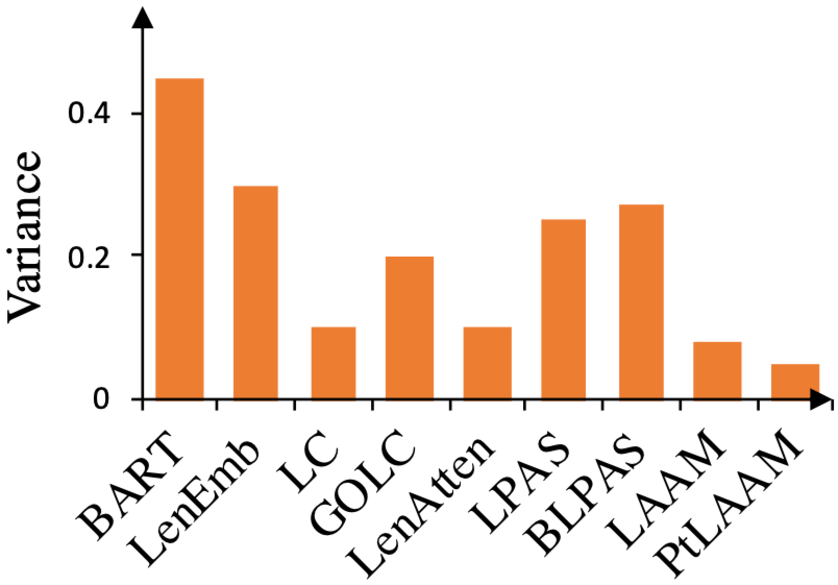
\includegraphics[width=1.4in]{allcnnvar.pdf}
		%\end{minipage}%
	}
	\subfigure[XSUM]{
	\label{fig:varX}
	%\begin{minipage}[t]{0.5\linewidth}
	\centering
	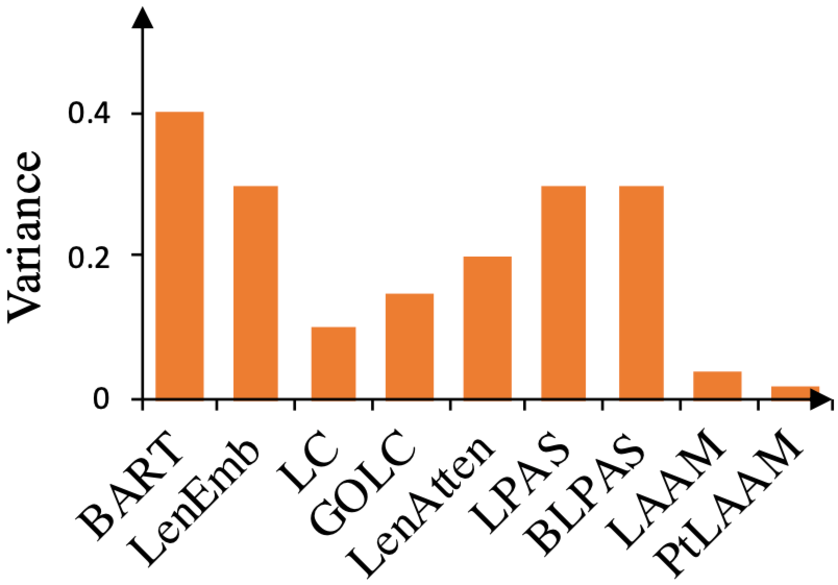
\includegraphics[width=1.4in]{allxvar.pdf}
	%\end{minipage}%
}
	\caption{Variance of generated summary lengths in gold length test with soft length control.}
	\label{fig:var}
\end{figure}

\begin{table}[th]
	\centering
	\scriptsize
	\begin{tabular}{|l|l|ccc|}
		\hline
		\bf Data & \bf Model & \bf Gram. & \bf Info. & \bf Overall \\
		\hline
		\multirow{3}{*}{CNNDM}&Gold& 4.6 & 4.3 & 4.1 \\
		&BART& 3.8 & 2.7 & 2.2 \\
		&BLPAS & 3.3 & 2.9 & 2.8  \\
	    &PtLAAM & 4.0 &3.4 & 3.3  \\
		\hline
		\multirow{3}{*}{XSUM}&Gold& 4.8 & 3.7 & 4.5 \\
		&BART& 3.0 & 2.9 & 2.0 \\
		&BLPAS & 2.1& 2.3 & 2.3 \\
		&PtLAAM & 3.4 & 3.0 & 2.9  \\
		\hline
	\end{tabular}
	\caption{Human evaluation. Average Cohen's Kappa is 0.62 among judges,
	indicating good agreement. }
	\label{tab:human}  
\end{table}

To further test the models' length control ability in
different target length ranges, we divide the test data into different sets according to 
length range in \tabref{tab:lendis}, and test the models on these sets separately.
\figref{fig:div_var_r} shows that LAAM and PtLAAM still achieve the lowest Var.
For the same length range in \figref{fig:div_var_r} and \tabref{tab:lendis}, the more training data in this range, the lower Var of the generated summaries with respect to the reference summaries within this length range.
This denotes that the imbalance length distribution in training data
interferes with controlling length.
In \figref{fig:div_var_r},
LAAM and PtLAAM have better and more stable ROUGE scores in all length ranges,
illustrating that our approaches are
not affected by the summary length distribution in training set 
and can generate better summaries with desired lengths.

\begin{figure}[!ht]
	\centering
	\scriptsize
	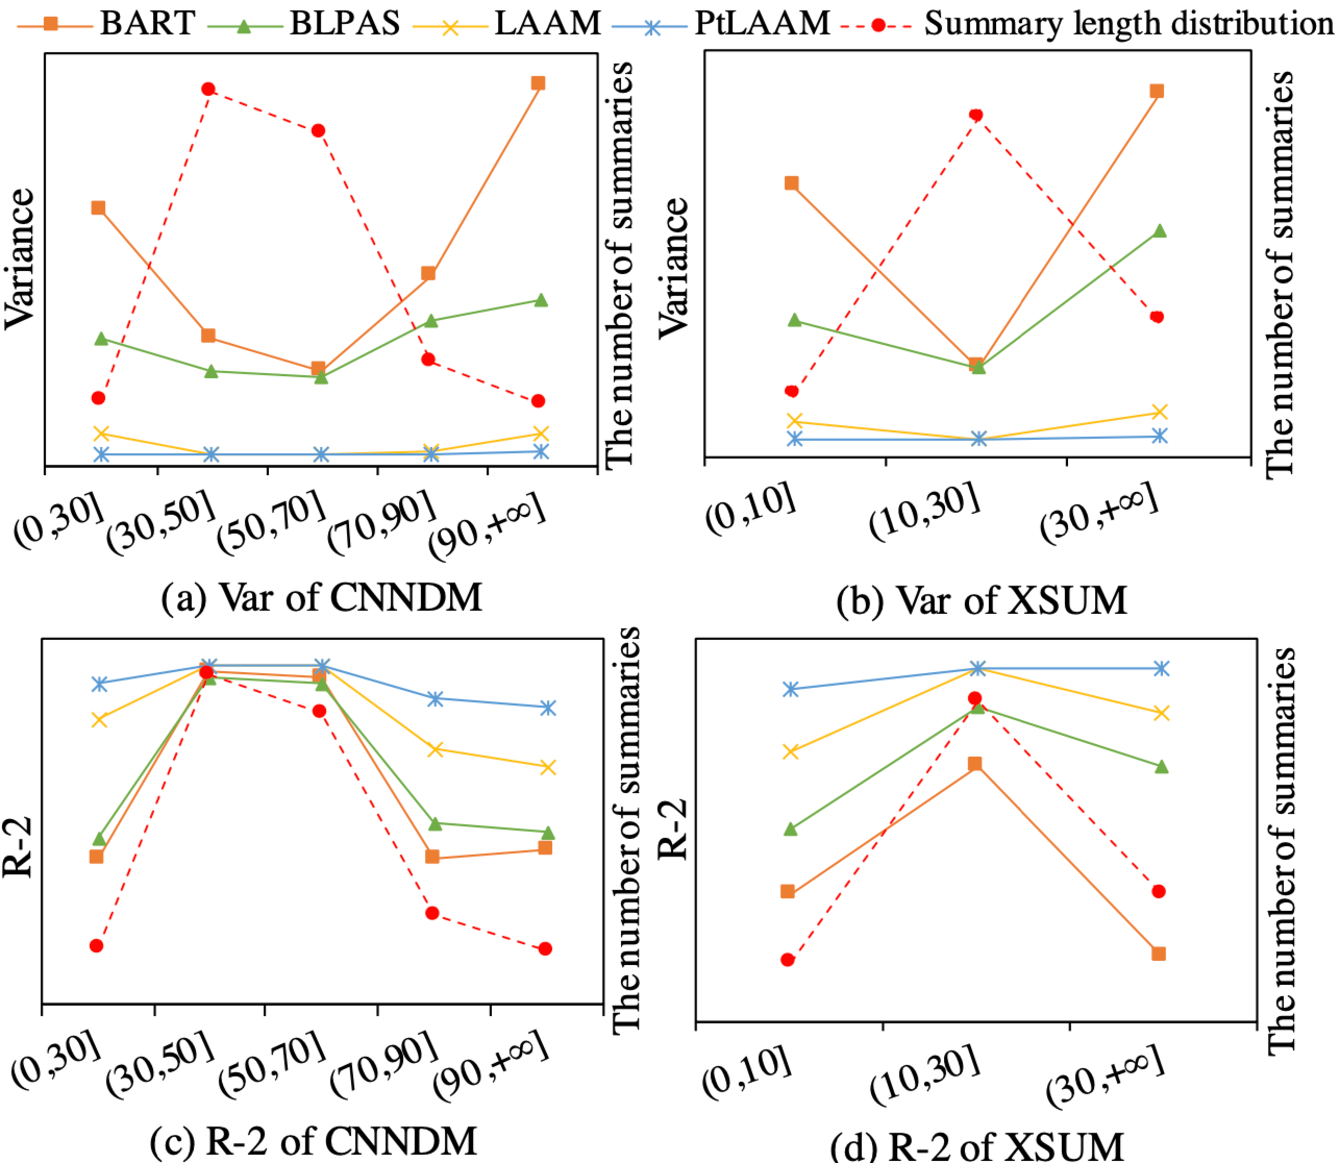
\includegraphics[width=1\linewidth]{div_var_r.pdf}
	\caption{Var and R-2(F1) scores of gold length test with soft length control on divided test sets.}
	\label{fig:div_var_r}
\end{figure}

The results of arbitrary length test are listed in \figref{fig:freearbi},
the lower Var of LAAM and PtLAAM illustrate our approach can control summary length better.
As R-2 is the most popular metric in summarization,
we report the R-2 related scores of generated summaries.
We compute R-2 Precision ({\bf Pre}) of generated summaries instead of F1, because 
when the desired length of generated summaries is shorter 
than reference summary lengths, precision can reflect the accuracy of 
information selection within that limited budget.
In \figref{fig:freearbi}, LAAM and PtLAAM get better R-2 (Pre) on both datasets, which means our approaches can select more accurate information. 
As the desired length increases, the length-controllable models are more likely to select accurate information,
causing the gap between our approach and BLPAS to gradually decrease.
Bart is not designed to control length, resulting in unchanged R-2 (Pre).
Although the arbitrary length test provides a unique perspective in
the evaluation of the models, its automatic metric, i.e., R-2 (Pre) is only partial.
Therefore, in the rest of the section, we will not do arbitrary length test
unless the result is evaluated by human.

\begin{figure}[!ht]
	\centering
	\scriptsize
	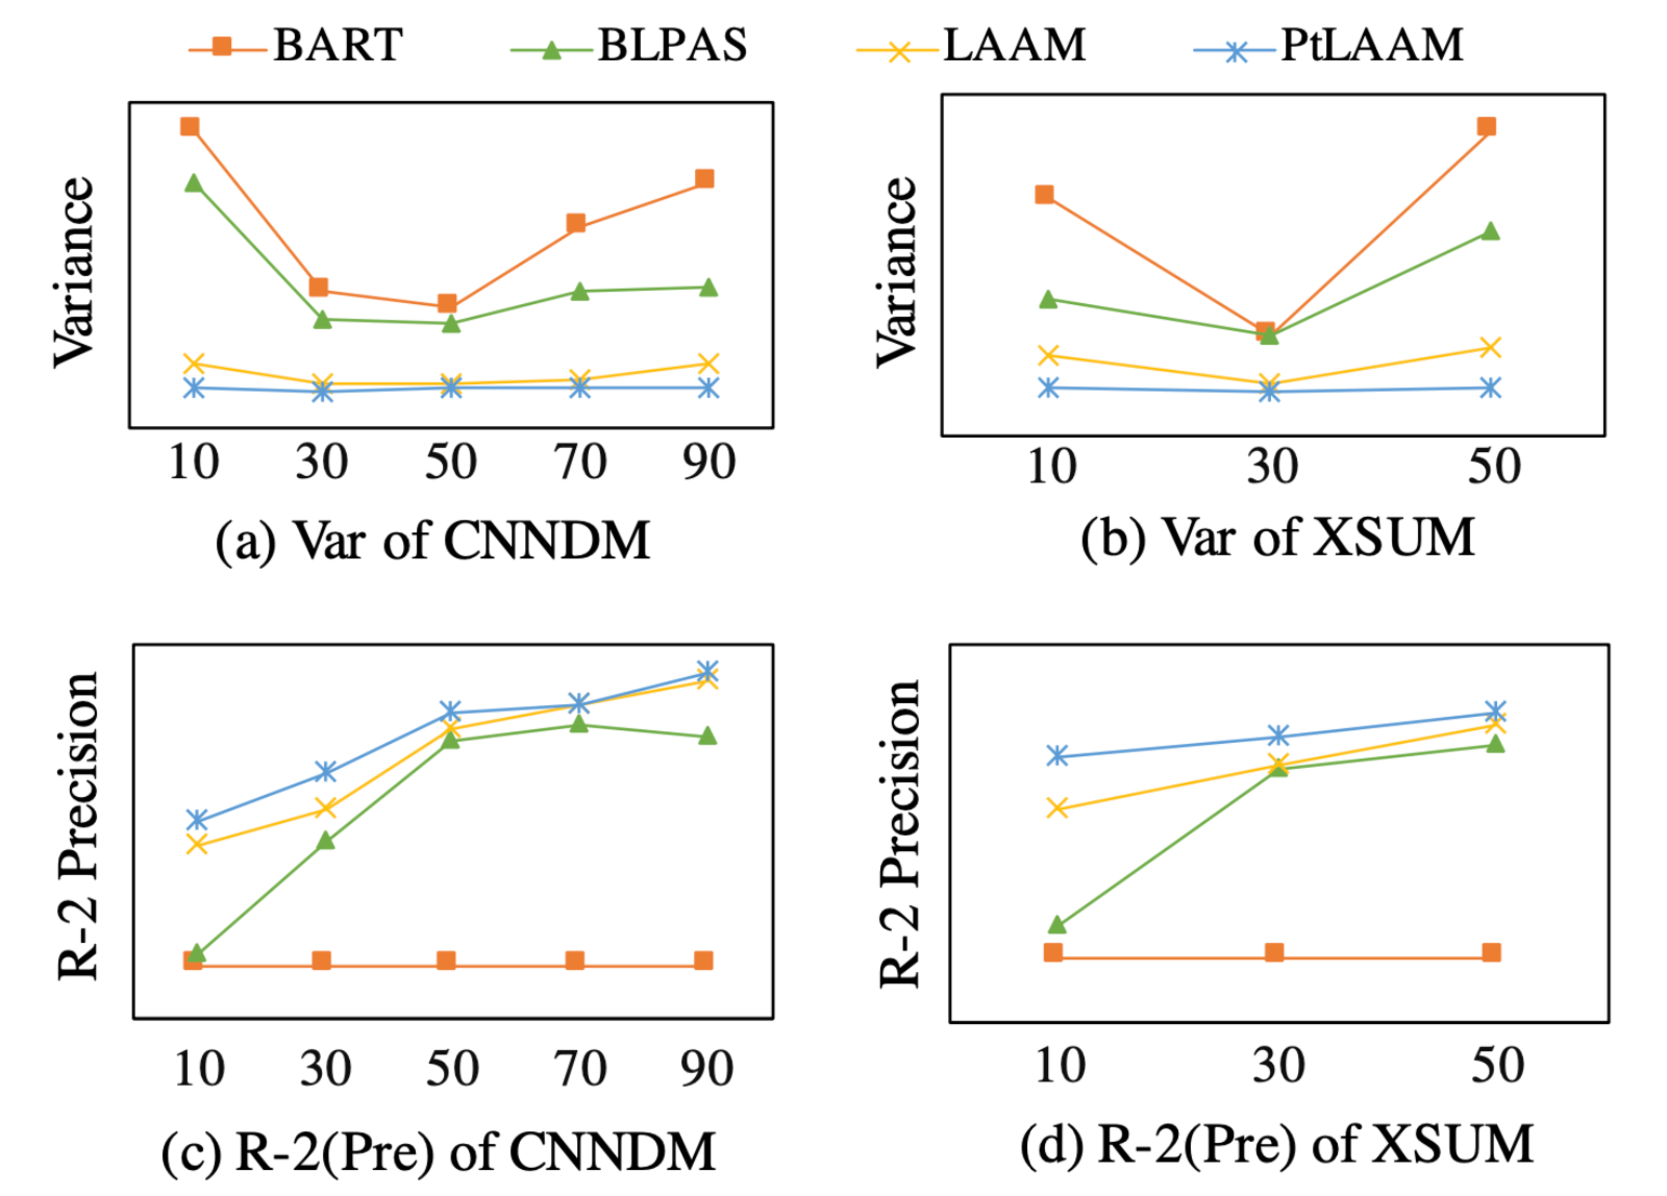
\includegraphics[width=0.95\linewidth]{freearbi.pdf}
	\caption{Var and R-2 (Pre) of arbitrary length test with soft length control on complete test sets.}
	\label{fig:freearbi}
\end{figure}

\textbf{Information selection.} 
Next, we apply hard length control on all models to strictly enforce the exact desired length which
is equal to the gold length.
The better performance of our proposed approaches in \tabref{tab:exact} indicates that our approaches can cover more important information while producing exactly the same length of the reference summary. 
Compared to \tabref{tab:genall}, our approaches also demonstrate more consistency.

\begin{table}[th]
	\centering
	\scriptsize
	\begin{tabular}{|m{0.8cm}<{\raggedleft}|p{0.45cm}<{\centering}|p{0.45cm}<{\centering}|p{0.45cm}<{\centering}|p{0.45cm}<{\centering}|p{0.45cm}<{\centering}|p{0.45cm}<{\centering}|}
		\hline
		\multirow{2}{*}{Approach} & \multicolumn{3}{c|}{\bf CNNDM} &  \multicolumn{3}{c|}{\bf XSUM} \\ \cline{2-7}
		 &R-1 & R-2 & R-L& R-1 & R-2 & R-L \\
		\hline
		 BART 
		            & 43.43& 20.11 & 39.52 & 44.82 & 21.34 & 36.23  \\
	  BLPAS & 43.15 & 20.52  & 40.01 &45.03 & 20.57 & 36.02  \\
       LAAM & 43.63 & 20.76 & 40.63 & 45.38 & 21.77 & 36.64 \\
     PtLAAM & \bf 44.21&\bf 20.77 &\bf 40.97  & \bf 45.53 &\bf 21.82 & \bf 36.85 \\
		\hline
	\end{tabular}
	\caption{The ROUGE scores of models in gold length test with hard length control. }\label{tab:exact}  
\end{table}

As shown in \tabref{tab:exp},
the summaries are generated by the SOTA length-controllable approach BLPAS 
and our best approach PtLAAM with desired length as $10$ tokens and $30$ tokens.
For BLPAS, the summary with desired length as $10$ is just the truncated version of the summary with desired length as $30$.
Different from BLPAS, the content of summaries generated by PtLAAM are changed according to different desired lengths, which denotes that PtLAAM is more effective in selecting information to be summarized by length constraint. 

\begin{table}[th!]
	\centering
	\scriptsize
	\begin{tabular}{|p{0.3cm}|p{3cm}|p{3cm}|}
		\hline 
         \bf Len & \bf BLPAS Summaries & \bf PtLAAM Summaries\\
		\hline 
		\bf 10 & \tabincell{l}{iranians erupted in celebration , \\ as young people waved flages } & \tabincell{l}{iranians celebrate online and in \\ the streets after deal .}\\
		\hline
		\bf 30 & \tabincell{l}{iranians erupted in celebration \\ as young people waved flages , \\ blasted music from stereos and \\ chatted online . the agreement \\ on the final day of persian new \\ year festivities .} 
		& \tabincell{l}{
		the excitement came after a \\ breakthrough nuclear deal with \\ the united states and other world \\powers . iranians erupted in \\celebration as young people \\ waved flags and chatted online .}
		\\
		\hline 
	\end{tabular}
	\caption{Generated summaries of two different lengths from the source document in \tabref{tab:intro}.\label{tab:exp} 
}
\end{table}


{\bf Ablation Studies.}We evaluate the effectiveness of the pretraining LAAM on LBD and length-aware attention mechanism.

\textit{Pretraining on LBD.} 
Compared with LAAM only training on original datasets, PtLAAM performs better on R-2 and Var in \figref{fig:freearbi} and \figref{fig:div_var_r}.
The better R-2 scores indicates that the PtLAAM can select more important information with pretrained LAAM on our created dataset LBD.
As one source document of LBD may have different extracted summaries within different length ranges, the model trained on LBD can learn to select different information from source document according to the length constraints.
Besides, in LBD, the number of summaries with lengths in different ranges is balanced.
PtLAAM gets lower Var, which denotes it can control length better.
The Var scores in different length ranges are stable, which 
weakens the negative impact caused by the imbalanced length distribution of training data. 

\textit{Length-aware attention mechanism,}
The length-aware attention consists of $Attn_{is}$ and $Attn_{eos}$.
\tabref{tab:lenattn} shows the results of LAAM test on gold length test with soft length control.
Compared with LAAM, 
the LAAM without $Attn_{is}$ has a big drop in ROUGE scores
and a small drop in Var score,
demonstrating that $Attn_{is}$ mainly focuses on select information with length constraint.
The LAAM without $Attn_{eos}$ gets the much lower Var scores but not much difference in ROUGE scores than LAAM,
which means that $Attn_{eos}$ is useful in limiting the output length.
LAAM outperforms its variant because of the effectiveness of length-aware attention mechanism. 
Thus, in our experiments, we use PtLAAM model, 
which trains LAAM with both $Attn_{is}$ and $Attn_{eos}$
on LBD first and then fine-tunes the original datasets, as our best approach.


\begin{table}[th]
	\centering
	\scriptsize
	\begin{tabular}{|c|lc|p{0.5cm}|p{0.5cm}|p{0.5cm}|p{0.6cm}<\centering|}
		\hline 
		Data & \multicolumn{2}{c|}{Model} & R-1 & R-2&R-L&Var(\%)\\
		\hline
		\multirow{3}{*}{CNNDM} & \multicolumn{2}{l|}{LAAM}  &\bf 43.63& \bf 20.76 & \bf 40.63 &\bf 0.05  \\ 
		&&w/o $Attn_{is}$ & 42.77 &  19.32 & 39.13 & 0.06\\
		&&w/o $Attn_{eos}$ & 43.10 &  20.17 & 37.45 & 0.13\\
		\hline
		\multirow{3}{*}{XSUM} &\multicolumn{2}{l|}{LAAM} & \bf 45.38 & \bf 21.77 & \bf 36.64& \bf 0.03 \\ 
		&&w/o $Attn_{is}$ & 43.45 & 20.64 & 34.79 & 0.03 \\
		&&w/o $Attn_{eos}$ & 44.62 &  21.32 & 35.03 & 0.08\\
		\hline
	\end{tabular}
	\caption{Usefulness of two kinds of attentions.} 
	\label{tab:lenattn}  
\end{table}


\subsection{Experiment 2: Zero-shot Length Control}
\label{sec:zeroshot}
In this experiment, 
we use the modified dataset for zero-shot length control (\secref{sec:expset}).
Zero-shot task can test a model's ability to generalize to 
summary lengths that it has never seen in the original training data before.

\begin{table}[th]
	\scriptsize
	\centering
	\begin{tabular}{|p{0.75cm}<\centering|p{0.65cm}<\centering|r|p{0.5cm}<\centering|p{0.5cm}<\centering|p{0.5cm}<\centering|p{0.55cm}<\centering|}
		\hline
		\bf Dataset& \bf Length &\bf Approach& \bf R-1 & \bf R-2 & \bf R-L &Var(\%) \\ 
		\hline
	    \multicolumn{7}{|c|}{\bf Soft length control }\\
	    \hline
		\multirow{3}{*}{CNNDM} 
		& \multirow{3}{*}{$(0,30]$} & BLPAS & 33.04 &14.83& 29.42 & 0.14 \\
		&& LAAM & 33.52 & 15.20 & 30.54 & 0.05 \\
		&& PtLAAM & \bf 33.65& \bf 15.77&\bf 31.26 & \bf 0.03\\
		\hline
		\multirow{3}{*}{XSUM} 
		& \multirow{3}{*}{$(0,10]$} & BLPAS & 34.37 & 19.54 & 31.66 & 0.10 \\
		&& LAAM & 34.49 &  20.07&32.10 & 0.03\\
		&& PtLAAM & \bf 35.16& \bf 20.55 & \bf 32.47 & \bf 0.02\\
		\hline
		\multicolumn{7}{|c|}{\bf Hard length control }\\
		\hline
		\multirow{3}{*}{CNNDM} 
		& \multirow{3}{*}{$(0,30]$} & BLPAS & 30.25 &12.51& 26.98 & -\\
		&& LAAM & 33.64 & 15.23 & 30.76 & - \\
		&& PtLAAM & \bf 33.78& \bf 15.89 &\bf 31.30 & \bf -\\	
				\hline	
		\multirow{3}{*}{XSUM} 
		& \multirow{3}{*}{$(0,10]$} & BLPAS & 32.55 & 17.16 & 29.52 & - \\
		&& LAAM & 34.83 &  20.15&32.10 & -\\
		&& PtLAAM & \bf 35.16& \bf 20.58 & \bf 32.49 & -\\
		\hline
	\end{tabular}
	\caption{Results of zero-shot length control.}\label{tab:zero}  
\end{table}

\tabref{tab:zero} shows the performance of PtLAAM on ROUGE scores and 
Var on different datatsets are the best.
For soft length control experiment,
the ROUGE scores of different models are similar,
because the lengths of summaries generated by BLPAS
are longer than reference summary lengths (BLPAS has higher Var scores), which causes the generated summaries 
to match more tokens in the reference.
Because ROUGE (F1) scores usually penalize summaries with longer lengths, 
PtLAAM, which controls the length better, is still better than other approaches.
The lowest Var of our approaches means that our approach can 
better control summary length.
In the hard length control experiment, the ROUGE scores of BLPAS drop a lot 
since the hard control shortens the length of summaries generated by BLPAS.
The best performance of PtLAAM on ROUGE indicate PtLAAM learns to select 
information based on desired lengths.
The ROUGE scores of our approaches are similar to those in 
soft length control experiment, which indicates our approaches are stable in controlling length.
The LAAM performs worse than PtLAAM on ROUGE and Var denotes that 
the ability of LAAM to control length is impacted by 
length distribution of the training data.
The pretraining on LBD is useful in 
generating high-quality summaries under desired summary length 
since the summaries are balanced in different length ranges of LBD.

\subsection{Case Study}
\label{sec:appendix}
In this section, we analyze the performance of different models in controlling length.

\begin{table}[th!]
	\centering
	\scriptsize
	\begin{tabular}{|p{0.3cm}|p{0.8cm}|p{4cm}|}
		\hline 
		\multicolumn{3}{|c|}{\bf Input Document} \\
		\hline
		\multicolumn{3}{|c|}{ \tabincell{l}{a gym teacher in new hampshire has been accused of posing as a young \\ girl on a social media site and persuading an elementary school student \\to share inappropriate images of herself ... police charged 34-year-old \\paul johnson-yarosevich of acton , maine , on monday with prohibited \\ use of computer after they say they discovered he 'd been fooling a \\ pre-teen girl into sending him inappropriate photos of herself by posing \\ as a young girl on social media . authorities soon learned that the girl \\ was sending the photos to a grown man ...}} \\
		\hline
		\hline 
		\bf Len & \multicolumn{2}{|c|}{\bf Generated summaries}  \\
		\hline
		-&\tabincell{l}{BART} & \tabincell{l}{police charged 34-year-old paul johnson-yarosevich \\ of acton , maine , on monday with prohibited use of \\computer after they say they discovered he 'd been \\fooling a pre-teen girl into sending him inappropriate \\ photos of herself by posing as a young girl on social \\ media . authorities soon learned that the girl was \\ sending the photos to a grown man .}  \\ \hline
		\multirow{4}{*}{\bf  $10$} & Exact & \tabincell{l}{police charged 34-year-old  paul johnson-yarosevich \\ of  acton , maine ,}  \\ \cline{2-3}
		& BLPAS & \tabincell{l}{police charged 34-year-old  paul johnson-yarosevich \\ of  acton with prohibited use \textcolor{red}{of a computer .}} \\\cline{2-3}
		&  LAAM & \tabincell{l}{paul was charged with prohibited use of a computer .} \\ \cline{2-3}
		& PtLAAM & \tabincell{l}{Paul was prohibited use of computer for cheating . }  \\
		\hline
		\multirow{4}{*}{\bf  $30$}  &Exact& \tabincell{l}{{\em police charged 34-year-old paul johnson-yarosevich} \\ {\em of acton , maine ,} on monday with prohibited use of \\computer after they say they discovered he 'd been \\fooling a pre-teen girl .} \\ \cline{2-3}
		&BLPAS& \tabincell{l}{\textit{police charged 34-year-old} \textit{paul johnson-yarosevich} \\ \textit{of acton , on monday with prohibited use of computer} \\ . the investigation started in december . after the \\ father of a pre-teen girl told \textcolor{red}{police about the contact .}
		} \\\cline{2-3}
		&LAAM&\tabincell{l}{police charged 34-year-old paul on monday
			with \\ prohibited use of computer after discovering he ’d \\ been fooling a girl into sending him inappropriate \\ photos of herself on social media . 
		}\\\cline{2-3}
		&PtLAAM& \tabincell{l}{police charged paul , 34 , on monday
			with prohibited \\ use of computer after discovering he ’d been fooling \\ a pre-teen girl into sending him inappropriate photos \\ on social media . 
		}
		\\\cline{2-3}
		
		\hline 
	\end{tabular}
	\caption{The generated summaries of \tabref{tab:intro} of various desired length \textbf{Len}. \label{tab:case} 
		The {\em italicized} tokens repeat significant parts
		the shorter summaries. The red is the tokens longer than desired length.Here Exact refers to the BART using Exact at test, to be fair.
	}
\end{table}

We use the example in \tabref{tab:case} to analyze different length-controllable methods since the summaries of this example generated by different models are obviously different in {\em length control} and {\em information selection}.

As shown in \tabref{tab:case}, BART itself cannot control the length of generated summaries.
So, the length of the summary generated by BART is always much longer for covering more information from source document. 
After adding Exact at test time, BART can generate summary with length exactly the same as desired length. But, as a {\em early-stop during decoding methods}, Exact always produce incomplete summaries. The summary with $30$ tokens of Exact repeats its summary with $10$ tokens during generation. Because such methods ignore that the summaries with different lengths of one document should represent different information of source document. 
BLPAS tends to select more information with length constraints, which may generate summaries with length longer than desired length (the red part in \tabref{tab:case}). 
The lengths of summaries generated by LAAM and PtLAAM in \tabref{tab:case} are the same as the desired lengths. 

Compared with PtLAAM, given the desired length as $10$, LAAM loses the important information about the reason why Paul was charged as there are few training pairs with summary lengths as $10$. PtLAAM pretrained on LBD can select information according to various desired lengths as the summary lengths in LBD are evenly distributed in different length ranges. The summaries with desired length as $30$ of LAAM and PtLAAM are more similar than their summaries with desired length as $10$. 
This is because there are many more summaries with length about $30$ than those with length about $10$ in original dataset. Thus, PtLAAM is more effective in generating summaries of lengths that do not appear in the original datasets.

